\documentclass{article}
\usepackage[utf8]{inputenc}
% are all of these packages really necessary?
% no.
% i'm just too lazy to only grab the packages i want for a specific
% document, so i just glob all of my most commonly used packages together
% this is bad practice.
\usepackage{amsmath,amsthm,amssymb,amsfonts, fancyhdr, color, comment, graphicx, environ, mdframed, soul, calc, enumitem, mdframed, xcolor, geometry, empheq, mathtools, tikz, pgfplots, caption, subcaption, hyperref}

\usetikzlibrary{external}
\tikzexternalize[prefix=tikz/,optimize command away=\includepdf]

%tikzpicture
\usepackage{tikz}
\usepackage{scalerel}
\usepackage{pict2e}
\usepackage{tkz-euclide}
\usetikzlibrary{calc}
\usetikzlibrary{patterns,arrows.meta}
\usetikzlibrary{shadows}
\usetikzlibrary{external}

%pgfplots
\usepackage{pgfplots}
\pgfplotsset{compat=newest}
\usepgfplotslibrary{statistics}
\usepgfplotslibrary{fillbetween}
\usepgfplotslibrary{polar}

\tikzset{external/export=true}
\pgfplotsset{
    standard/.style={
    axis line style = thick,
    trig format=rad,
    enlargelimits,
    axis x line=middle,
    axis y line=middle,
    enlarge x limits=0.15,
    enlarge y limits=0.15,
    every axis x label/.style={at={(current axis.right of origin)},anchor=north west},
    every axis y label/.style={at={(current axis.above origin)},anchor=south east}
    }
}
\newcommand*\widefbox[1]{\fbox{\hspace{2em}#1\hspace{2em}}}
% Command "alignedbox{}{}" for a box within an align environment
% Source: http://www.latex-community.org/forum/viewtopic.php?f=46&t=8144
\newlength\dlf  % Define a new measure, dlf
\newcommand\alignedbox[2]{
% Argument #1 = before & if there were no box (lhs)
% Argument #2 = after & if there were no box (rhs)
&  % Alignment sign of the line
{
\settowidth\dlf{$\displaystyle #1$}  
    % The width of \dlf is the width of the lhs, with a displaystyle font
\addtolength\dlf{\fboxsep+\fboxrule}  
    % Add to it the distance to the box, and the width of the line of the box
\hspace{-\dlf}  
    % Move everything dlf units to the left, so that & #1 #2 is aligned under #1 & #2
\boxed{#1 #2}
    % Put a box around lhs and rhs
}
}

\hypersetup{
    colorlinks=true,
    linkcolor=blue,
    filecolor=magenta,      
    urlcolor=cyan,
    pdftitle={Homework 12 Solutions},
    pdfpagemode=UseOutlines,
    bookmarksopen=true,
    pdfauthor={Christina Phan}
}
\newcommand{\lrp}[1]{\left( #1 \right)}
\newcommand{\abs}[1]{\left\vert #1 \right\vert}
\newcommand{\lra}[1]{\left\langle #1 \right\rangle}
\newcommand{\lrb}[1]{\left[ #1 \right]}
\newcommand{\norm}[1]{\left\lVert #1 \right\rVert}
\newcommand{\iintR}[0]{\iint\limits_{R}}
\renewcommand{\u}[0]{\mathbf{u}}
\renewcommand{\i}[0]{\mathbf{i}}
\renewcommand{\j}[0]{\mathbf{j}}
\renewcommand{\k}[0]{\mathbf{k}}
\newcommand{\T}[0]{\mathbf{T}}
\newcommand{\N}[0]{\mathbf{N}}
\newcommand{\B}[0]{\mathbf{B}}
\renewcommand{\r}[0]{\mathbf{r}}
\renewcommand{\a}[0]{\mathbf{a}}
\renewcommand{\v}[0]{\mathbf{v}}
\newcommand{\F}[0]{\mathbf{F}}

\geometry{letterpaper, portrait, margin=1in}
\renewcommand{\footrulewidth}{0.8pt}
\setlength\parindent{0pt}
\pagestyle{fancy}
\lhead{Christina Phan}
\rhead{MAT 21D} 
\chead{\textbf{Homework 12 Solutions}}

\newcommand{\Solution}{\textit{Solution}}
\pgfplotsset{compat=1.18}
\begin{document}
\phantomsection
\addcontentsline{toc}{section}{Problem 1}\textbf{Problem 1}

Find a formula $\F(x,y)=\lra{M(x,y), N(x,y)}$ for the vector field with the property that $\F$ points toward the origin with magnitude inversely proportional to the square of the
distance from $(x, y)$ to the origin. (The field is not defined at the origin.)

\Solution

Recall that a vector consist of a magnitude and a direction.

For the magnitude, we're told that the magnitude of $\F(x,y)$ is inversely proportional to the square of the distance from $(x,y)$ to the origin. That is,
\begin{align*}
    \norm{\F(x,y)}&=\frac{k}{x^2+y^2}\tag{$\text{dist}=\sqrt{(x-0)^2+(y-0)^2}$}
\end{align*}
where $k$ is some constant greater than $0$ since magnitude (length) can never be negative.

We can get the direction of $\F(x,y)$ pretty easily as well. The unit vector of $\F(x,y)$ is going to be in the direction of $\lra{-x,-y}$ because we're pointing \textit{towards} the origin. 

Hopefully the figures below make it a bit more clear. When we have $\F(x,y)=\lra{x,y}$ the vectors are pointing \textit{away} from the origin. We want the vectors to point \textit{towards} the origin, so we multiply the vectors by $-1$ (flip the direction). If we multiply the vectors by $-1$, then $\F(x,y)=-\lra{x,y}=\lra{-x,-y}$.
\begin{figure}[h]
\centering
\begin{minipage}{.5\textwidth}
  \centering
  

\tikzset{every picture/.style={line width=0.75pt}} %set default line width to 0.75pt        

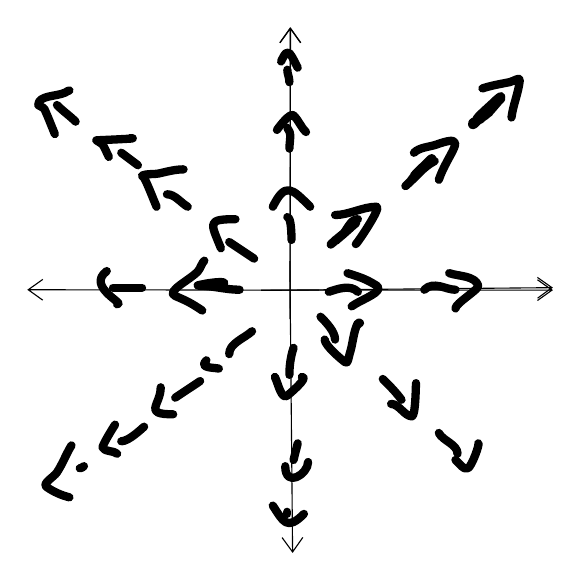
\begin{tikzpicture}[x=0.75pt,y=0.75pt,yscale=-1,xscale=1]
%uncomment if require: \path (0,300); %set diagram left start at 0, and has height of 300

%Shape: Axis 2D [id:dp7100385569457184] 
\draw  (247,146.98) -- (387.2,146.98)(261.02,20.8) -- (261.02,161) (380.2,141.98) -- (387.2,146.98) -- (380.2,151.98) (256.02,27.8) -- (261.02,20.8) -- (266.02,27.8)  ;
%Shape: Axis 2D [id:dp9010325381036207] 
\draw  (261,161) -- (261.2,20.8)(134.84,146.8) -- (275.04,147) (256.19,27.79) -- (261.2,20.8) -- (266.19,27.81) (141.83,151.81) -- (134.84,146.8) -- (141.85,141.81)  ;
%Shape: Axis 2D [id:dp896038649218499] 
\draw  (260.89,132.96) -- (262.21,273.15)(387.19,145.79) -- (247,147.11) (267.14,266.11) -- (262.21,273.15) -- (257.14,266.2) (380.15,140.86) -- (387.19,145.79) -- (380.24,150.86)  ;
%Shape: Free Drawing [id:dp843901335742354] 
\draw  [line width=3] [line join = round][line cap = round] (293.67,112.8) .. controls (289.9,112.8) and (288.49,118.29) .. (285.67,120.8) .. controls (284.07,122.22) and (279.16,126.31) .. (280.67,124.8) .. controls (282.84,122.63) and (285.35,120.82) .. (287.67,118.8) .. controls (289.27,117.39) and (294.31,113.43) .. (292.67,114.8) .. controls (289.94,117.07) and (287.43,119.59) .. (284.67,121.8) .. controls (282.79,123.3) and (282.67,123.91) .. (282.67,122.8) ;
%Shape: Free Drawing [id:dp24025447306937653] 
\draw  [line width=3] [line join = round][line cap = round] (282.67,110.8) .. controls (289.22,110.8) and (296.08,106.8) .. (302.67,106.8) .. controls (305.41,106.8) and (292.67,125.45) .. (292.67,124.8) ;
%Shape: Free Drawing [id:dp5933490017702595] 
\draw  [line width=3] [line join = round][line cap = round] (330.67,84.8) .. controls (325.17,87.55) and (321.39,92.87) .. (316.67,96.8) .. controls (315.94,97.4) and (318,95.47) .. (318.67,94.8) .. controls (319.85,93.62) and (320.49,91.98) .. (321.67,90.8) .. controls (322.6,89.87) and (329.67,85.36) .. (329.67,83.8) .. controls (329.67,82.13) and (326.91,85.69) .. (325.67,86.8) .. controls (323.91,88.37) and (322.18,89.99) .. (320.67,91.8) .. controls (320.67,91.8) and (320.67,94.47) .. (320.67,91.8) ;
%Shape: Free Drawing [id:dp009745257443489308] 
\draw  [line width=3] [line join = round][line cap = round] (320.67,80.8) .. controls (323.43,78.04) and (327.99,78.11) .. (331.67,76.8) .. controls (348.55,70.77) and (336.9,81.1) .. (332.67,93.8) ;
%Shape: Free Drawing [id:dp9162076713811873] 
\draw  [line width=3] [line join = round][line cap = round] (354.67,61.8) .. controls (352.83,63.64) and (348.67,69.4) .. (348.67,66.8) .. controls (348.67,65.31) and (351.43,65.63) .. (352.67,64.8) .. controls (354.83,63.36) and (355.83,60.64) .. (357.67,58.8) .. controls (359.18,57.29) and (364.18,53.29) .. (362.67,54.8) .. controls (359.16,58.3) and (356.37,63.23) .. (351.67,64.8) .. controls (347.86,66.07) and (356.83,58.64) .. (359.67,55.8) .. controls (360.52,54.95) and (363.2,52.73) .. (362.67,53.8) .. controls (361.13,56.88) and (358.21,58.72) .. (356.67,61.8) ;
%Shape: Free Drawing [id:dp7231284475896693] 
\draw  [line width=3] [line join = round][line cap = round] (353.67,49.8) .. controls (357.89,48.39) and (362.31,47.67) .. (366.67,46.8) .. controls (368.33,46.47) and (371.84,44.11) .. (371.67,45.8) .. controls (371.06,51.92) and (368.43,57.7) .. (367.67,63.8) ;
%Shape: Free Drawing [id:dp9213266096608321] 
\draw  [line width=3] [line join = round][line cap = round] (275.67,159.8) .. controls (278.33,162.46) and (282.67,167.01) .. (282.67,170.8) ;
%Shape: Free Drawing [id:dp13896247990407073] 
\draw  [line width=3] [line join = round][line cap = round] (305.67,189.8) .. controls (308.84,192.97) and (312.06,196.15) .. (314.67,199.8) ;
%Shape: Free Drawing [id:dp02437313111075956] 
\draw  [line width=3] [line join = round][line cap = round] (332.67,215.8) .. controls (334.57,219.6) and (341.67,221.27) .. (341.67,225.8) ;
%Shape: Free Drawing [id:dp7712158379605242] 
\draw  [line width=3] [line join = round][line cap = round] (277.67,170.8) .. controls (277.67,173.73) and (286.22,180.83) .. (287.67,181.8) .. controls (288.91,182.63) and (289.2,179.21) .. (289.67,177.8) .. controls (291.3,172.89) and (291.35,167.43) .. (293.67,162.8) .. controls (293.82,162.5) and (294.67,162.8) .. (294.67,162.8) .. controls (294.67,162.8) and (293.67,162.47) .. (293.67,163.8) ;
%Shape: Free Drawing [id:dp371019531436269] 
\draw  [line width=3] [line join = round][line cap = round] (309.67,201.8) .. controls (313.45,201.8) and (316.22,207.8) .. (319.67,207.8) .. controls (321.46,207.8) and (321.55,193.39) .. (321.67,191.8) ;
%Shape: Free Drawing [id:dp33226455240624286] 
\draw  [line width=3] [line join = round][line cap = round] (340.67,228.8) .. controls (342.54,230.3) and (344.52,233.87) .. (346.67,232.8) .. controls (348.62,231.82) and (352.52,220.8) .. (351.67,220.8) ;
%Shape: Free Drawing [id:dp3112565966036306] 
\draw  [line width=3] [line join = round][line cap = round] (242.67,166.8) .. controls (238.83,170.29) and (231.67,172.61) .. (231.67,177.8) ;
%Shape: Free Drawing [id:dp37653353016193714] 
\draw  [line width=3] [line join = round][line cap = round] (217.67,190.8) .. controls (213.67,193.47) and (209.67,196.13) .. (205.67,198.8) ;
%Shape: Free Drawing [id:dp21576613332986738] 
\draw  [line width=3] [line join = round][line cap = round] (190.67,212.8) .. controls (189.52,213.66) and (183.39,219.8) .. (179.67,219.8) ;
%Shape: Free Drawing [id:dp004016800357819816] 
\draw  [line width=3] [line join = round][line cap = round] (161.67,231.8) .. controls (161.14,232.33) and (160.41,232.8) .. (159.67,232.8) ;
%Shape: Free Drawing [id:dp7448281815981996] 
\draw  [line width=3] [line join = round][line cap = round] (155.67,221.8) .. controls (153.06,225.97) and (151.4,230.7) .. (148.67,234.8) .. controls (147.08,237.19) and (141.33,240.13) .. (143.67,241.8) .. controls (146.94,244.14) and (150.76,245.82) .. (154.67,246.8) ;
%Shape: Free Drawing [id:dp7475845335384022] 
\draw  [line width=3] [line join = round][line cap = round] (176.67,211.8) .. controls (175.51,213.54) and (170.3,222.06) .. (170.67,222.8) .. controls (171.8,225.08) and (176.01,224.15) .. (177.67,225.8) ;
%Shape: Free Drawing [id:dp7037868873659768] 
\draw  [line width=3] [line join = round][line cap = round] (198.67,193.8) .. controls (198.67,202.45) and (189.72,206.8) .. (204.67,206.8) ;
%Shape: Free Drawing [id:dp33398774070693427] 
\draw  [line width=3] [line join = round][line cap = round] (220.67,180.8) .. controls (216.77,184.7) and (224.22,184.19) .. (226.67,184.8) ;
%Shape: Free Drawing [id:dp5929100707222632] 
\draw  [line width=3] [line join = round][line cap = round] (243.67,131.8) .. controls (239.67,129.13) and (235.67,126.47) .. (231.67,123.8) ;
%Shape: Free Drawing [id:dp13852952101089788] 
\draw  [line width=3] [line join = round][line cap = round] (211.67,106.8) .. controls (208.29,104.87) and (205.55,100.8) .. (201.67,100.8) ;
%Shape: Free Drawing [id:dp33226882256343615] 
\draw  [line width=3] [line join = round][line cap = round] (187.67,86.8) .. controls (185,84.8) and (182.33,82.8) .. (179.67,80.8) ;
%Shape: Free Drawing [id:dp06998546523013494] 
\draw  [line width=3] [line join = round][line cap = round] (157.67,65.8) .. controls (154.67,62.8) and (151.88,61.01) .. (148.67,57.8) ;
%Shape: Free Drawing [id:dp6051596705819102] 
\draw  [line width=3] [line join = round][line cap = round] (147.67,71.8) .. controls (146,67.8) and (144.48,63.73) .. (142.67,59.8) .. controls (142.26,58.93) and (139.67,58.03) .. (139.67,57.8) .. controls (139.67,53.03) and (148.33,53.8) .. (152.67,51.8) .. controls (153.34,51.49) and (153.92,50.8) .. (154.67,50.8) ;
%Shape: Free Drawing [id:dp7029157312149265] 
\draw  [line width=3] [line join = round][line cap = round] (173.67,82.8) .. controls (172.67,80.8) and (171.85,78.7) .. (170.67,76.8) .. controls (170.58,76.66) and (167.67,74.8) .. (167.67,74.8) .. controls (167.67,74.8) and (191.42,73.8) .. (183.67,73.8) ;
%Shape: Free Drawing [id:dp13377978211608943] 
\draw  [line width=3] [line join = round][line cap = round] (196.67,106.8) .. controls (194.67,102.13) and (192.94,97.34) .. (190.67,92.8) .. controls (190.46,92.38) and (189.25,92.01) .. (189.67,91.8) .. controls (191.72,90.77) and (195.44,91.3) .. (197.67,90.8) .. controls (201.63,89.92) and (205.61,88.8) .. (209.67,88.8) ;
%Shape: Free Drawing [id:dp6231296734846898] 
\draw  [line width=3] [line join = round][line cap = round] (227.67,126.8) .. controls (222.75,114.51) and (220.6,112.8) .. (234.67,112.8) ;
%Shape: Free Drawing [id:dp33682607275124354] 
\draw  [line width=3] [line join = round][line cap = round] (236.67,146.8) .. controls (229.93,146.8) and (223.46,144.8) .. (216.67,144.8) .. controls (215.29,144.8) and (219.32,144.07) .. (220.67,143.8) .. controls (222.09,143.52) and (233.44,141.92) .. (227.67,144.8) ;
%Shape: Free Drawing [id:dp9331819401921526] 
\draw  [line width=3] [line join = round][line cap = round] (219.67,132.8) .. controls (218.29,134.17) and (217.93,136.32) .. (216.67,137.8) .. controls (213.14,141.92) and (200.68,147.66) .. (205.67,149.8) .. controls (211.79,152.42) and (213.45,153.32) .. (218.67,156.8) ;
%Shape: Free Drawing [id:dp23899385093465209] 
\draw  [line width=3] [line join = round][line cap = round] (189.67,145.8) .. controls (185,145.8) and (180.33,145.8) .. (175.67,145.8) ;
%Shape: Free Drawing [id:dp11471023636580935] 
\draw  [line width=3] [line join = round][line cap = round] (172.67,137.8) .. controls (162.54,145.4) and (182.25,153.8) .. (177.67,153.8) ;
%Shape: Free Drawing [id:dp04389787886335106] 
\draw  [line width=3] [line join = round][line cap = round] (279.67,147.8) .. controls (284,146.36) and (290.04,144.17) .. (293.67,147.8) ;
%Shape: Free Drawing [id:dp646145538331171] 
\draw  [line width=3] [line join = round][line cap = round] (288.67,138.8) .. controls (294.5,140.74) and (297.02,141.27) .. (302.67,144.8) .. controls (307.08,147.56) and (294.83,151.68) .. (290.67,154.8) ;
%Shape: Free Drawing [id:dp5958022333196401] 
\draw  [line width=3] [line join = round][line cap = round] (325.67,146.8) .. controls (330.17,142.29) and (335.93,146.8) .. (340.67,146.8) ;
%Shape: Free Drawing [id:dp008550406986449932] 
\draw  [line width=3] [line join = round][line cap = round] (337.67,138.8) .. controls (342.48,140.41) and (350.06,139.98) .. (351.67,144.8) .. controls (352.26,146.57) and (340.67,153.27) .. (340.67,155.8) ;
%Shape: Free Drawing [id:dp5697838340189935] 
\draw  [line width=3] [line join = round][line cap = round] (261.67,122.8) .. controls (261.67,121.75) and (261.74,111.8) .. (259.67,111.8) ;
%Shape: Free Drawing [id:dp14681013040478863] 
\draw  [line width=3] [line join = round][line cap = round] (252.67,106.8) .. controls (258.8,94.53) and (261.94,98.07) .. (270.67,106.8) ;
%Shape: Free Drawing [id:dp5066548038423898] 
\draw  [line width=3] [line join = round][line cap = round] (260.67,78.8) .. controls (260.67,75.45) and (262.04,71.17) .. (259.67,68.8) ;
%Shape: Free Drawing [id:dp4836235741631123] 
\draw  [line width=3] [line join = round][line cap = round] (254.67,69.8) .. controls (255.47,68.6) and (261.03,61.17) .. (262.67,62.8) .. controls (265.45,65.58) and (265.88,68.02) .. (268.67,70.8) ;
%Shape: Free Drawing [id:dp1738121935529453] 
\draw  [line width=3] [line join = round][line cap = round] (260.67,46.8) .. controls (260.67,44.32) and (259.67,43) .. (259.67,40.8) ;
%Shape: Free Drawing [id:dp12585429425718675] 
\draw  [line width=3] [line join = round][line cap = round] (256.67,36.8) .. controls (256.75,36.68) and (259.03,30.89) .. (260.67,32.8) .. controls (262.42,34.84) and (263.33,37.47) .. (264.67,39.8) ;
%Shape: Free Drawing [id:dp9672792538848222] 
\draw  [line width=3] [line join = round][line cap = round] (262.67,174.8) .. controls (261.28,178.96) and (260.67,183.42) .. (260.67,187.8) ;
%Shape: Free Drawing [id:dp34773854347885813] 
\draw  [line width=3] [line join = round][line cap = round] (253.67,188.8) .. controls (255.28,192.02) and (256.78,199.96) .. (259.67,197.8) .. controls (260.09,197.48) and (270.54,188.8) .. (266.67,188.8) ;
%Shape: Free Drawing [id:dp618713100718457] 
\draw  [line width=3] [line join = round][line cap = round] (264.67,220.8) .. controls (264,223.47) and (263.33,226.13) .. (262.67,228.8) ;
%Shape: Free Drawing [id:dp9029416369954855] 
\draw  [line width=3] [line join = round][line cap = round] (258.67,231.8) .. controls (258.67,242.6) and (269.67,235.64) .. (269.67,229.8) ;
%Shape: Free Drawing [id:dp8272687523240728] 
\draw  [line width=3] [line join = round][line cap = round] (259.67,253.8) .. controls (259.67,254.13) and (259.67,254.47) .. (259.67,254.8) ;
%Shape: Free Drawing [id:dp6600581922357868] 
\draw  [line width=3] [line join = round][line cap = round] (252.67,250.8) .. controls (257.78,258.47) and (259.34,263.13) .. (267.67,254.8) ;




\end{tikzpicture}
  \caption*{graph of $\frac{1}{\sqrt{x^2+y^2}}\lra{x,y}$}
  \label{fig:test1}
\end{minipage}%
\begin{minipage}{.5\textwidth}
  \centering
  

\tikzset{every picture/.style={line width=0.75pt}} %set default line width to 0.75pt        

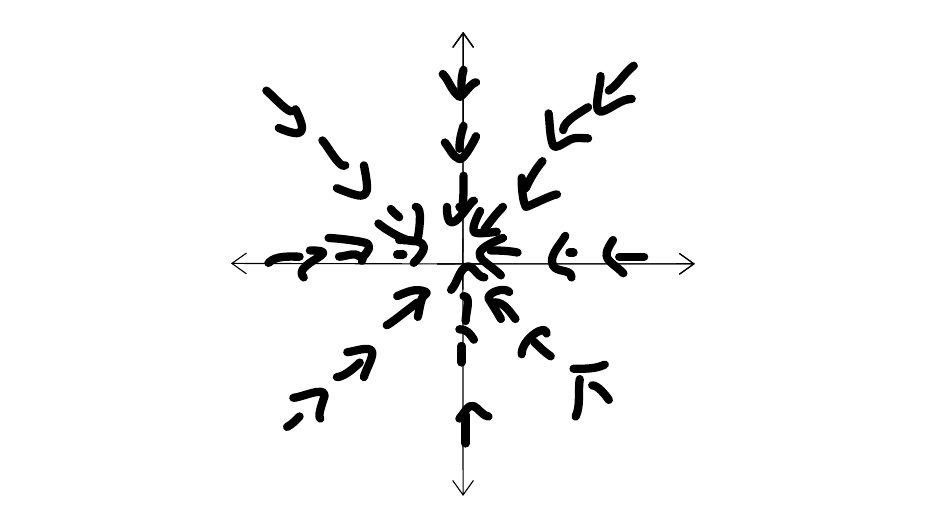
\begin{tikzpicture}[x=0.75pt,y=0.75pt,yscale=-1,xscale=1]
%uncomment if require: \path (0,300); %set diagram left start at 0, and has height of 300

%Shape: Axis 2D [id:dp13914496466940185] 
\draw  (269,138.63) -- (392.67,138.63)(281.37,27.33) -- (281.37,151) (385.67,133.63) -- (392.67,138.63) -- (385.67,143.63) (276.37,34.33) -- (281.37,27.33) -- (286.37,34.33)  ;
%Shape: Axis 2D [id:dp6909326742441152] 
\draw  (281.34,151) -- (281.62,27.33)(170.07,138.38) -- (293.73,138.66) (276.6,34.32) -- (281.62,27.33) -- (286.6,34.34) (177.06,143.4) -- (170.07,138.38) -- (177.08,133.4)  ;
%Shape: Axis 2D [id:dp6095404425634481] 
\draw  (281.36,126.27) -- (281.44,249.93)(392.67,138.56) -- (269,138.64) (286.44,242.93) -- (281.44,249.93) -- (276.44,242.94) (385.66,133.56) -- (392.67,138.56) -- (385.67,143.56)  ;
%Shape: Free Drawing [id:dp8613151098236289] 
\draw  [draw opacity=0][line width=3] [line join = round][line cap = round] (307.67,111.8) .. controls (306.22,113.97) and (304.51,115.96) .. (302.67,117.8) ;
%Shape: Free Drawing [id:dp9272206567111847] 
\draw  [draw opacity=0][line width=3] [line join = round][line cap = round] (308.67,110.8) .. controls (306.67,114.47) and (304.67,118.13) .. (302.67,121.8) ;
%Shape: Free Drawing [id:dp8213114496949026] 
\draw  [draw opacity=0][line width=3] [line join = round][line cap = round] (301.67,117.8) .. controls (299.32,121.33) and (297.61,125.85) .. (294.67,128.8) ;
%Shape: Free Drawing [id:dp33907945921125693] 
\draw  [draw opacity=0][line width=3] [line join = round][line cap = round] (310.67,109.8) .. controls (305.97,113.32) and (301.94,117.9) .. (298.67,122.8) ;
%Shape: Free Drawing [id:dp428873025263114] 
\draw  [draw opacity=0][line width=3] [line join = round][line cap = round] (317.67,105.8) .. controls (314.33,109.47) and (310.67,112.86) .. (307.67,116.8) .. controls (305.2,120.04) and (300.67,130.87) .. (300.67,126.8) ;
%Shape: Free Drawing [id:dp34273800045821023] 
\draw  [draw opacity=0][line width=3] [line join = round][line cap = round] (312.67,109.8) .. controls (306.98,113.59) and (302.24,118.72) .. (297.67,123.8) ;
%Shape: Free Drawing [id:dp7359912846079759] 
\draw  [draw opacity=0][line width=3] [line join = round][line cap = round] (310.67,108.8) .. controls (306.42,111.35) and (297.67,115.4) .. (297.67,120.8) ;
%Shape: Free Drawing [id:dp562556916637904] 
\draw  [draw opacity=0][line width=3] [line join = round][line cap = round] (315.67,106.8) .. controls (310.31,111.26) and (304.57,115.9) .. (299.67,120.8) .. controls (293.45,127.02) and (293.67,130.99) .. (293.67,126.8) ;
%Shape: Free Drawing [id:dp16548347665626117] 
\draw  [draw opacity=0][line width=3] [line join = round][line cap = round] (496.67,75.8) .. controls (498.27,95.08) and (497.3,114.63) .. (494.67,133.8) .. controls (493.88,139.5) and (493.01,145.2) .. (491.67,150.8) .. controls (491.04,153.41) and (489.57,159.7) .. (487.67,157.8) ;
%Shape: Free Drawing [id:dp7680735814954041] 
\draw  [draw opacity=0][line width=3] [line join = round][line cap = round] (73.67,232.8) .. controls (77.18,212.89) and (83.83,194.69) .. (101.67,182.8) .. controls (107.42,178.97) and (115.06,176.07) .. (120.67,182.8) .. controls (130.25,194.3) and (100.18,229.32) .. (88.67,217.8) .. controls (76.15,205.28) and (91.2,166.57) .. (99.67,155.8) .. controls (104.15,150.09) and (115.8,140.4) .. (124.67,146.8) .. controls (142.65,159.79) and (122.28,191.85) .. (114.67,201.8) .. controls (109.92,208.01) and (97.98,217.23) .. (88.67,213.8) .. controls (81.98,211.33) and (82.47,190.78) .. (82.67,188.8) .. controls (84.47,170.31) and (90.7,138.06) .. (111.67,130.8) .. controls (119.54,128.07) and (131.88,129.35) .. (132.67,140.8) .. controls (133.68,155.53) and (121.48,174.8) .. (105.67,174.8) ;
%Shape: Free Drawing [id:dp07144523007812364] 
\draw  [draw opacity=0][line width=3] [line join = round][line cap = round] (304.67,112.8) .. controls (304.67,118.97) and (298.21,121.26) .. (294.67,124.8) ;
%Shape: Free Drawing [id:dp6112173073386881] 
\draw  [draw opacity=0][line width=3] [line join = round][line cap = round] (315.67,94.8) .. controls (315.67,105.7) and (299.67,112.44) .. (299.67,121.8) ;
%Shape: Free Drawing [id:dp7654610054563705] 
\draw  [draw opacity=0][line width=3] [line join = round][line cap = round] (240.67,170.8) .. controls (241.67,170.13) and (242.75,169.58) .. (243.67,168.8) .. controls (245.52,167.21) and (259.67,155.33) .. (259.67,158.8) ;
%Shape: Free Drawing [id:dp9731876263438487] 
\draw  [draw opacity=0][line width=3] [line join = round][line cap = round] (236.67,185.8) .. controls (243.91,175.66) and (251.16,167.3) .. (260.67,158.8) .. controls (262.61,157.06) and (264.83,155.64) .. (266.67,153.8) .. controls (266.9,153.56) and (267.87,153.54) .. (267.67,153.8) .. controls (262.59,160.33) and (244.95,180.66) .. (235.67,178.8) .. controls (233.18,178.3) and (237.14,173.83) .. (238.67,171.8) .. controls (240.51,169.34) and (242.41,166.88) .. (244.67,164.8) .. controls (253.5,156.65) and (279.6,128.27) .. (296.67,136.8) .. controls (313.7,145.32) and (305.04,176.67) .. (295.67,187.8) .. controls (294.44,189.25) and (286,198.76) .. (280.67,195.8) .. controls (268.83,189.22) and (278.01,163.23) .. (281.67,154.8) .. controls (292.76,129.19) and (332.17,83.14) .. (364.67,104.8) ;
%Shape: Free Drawing [id:dp5021887877278205] 
\draw  [draw opacity=0][line width=3] [line join = round][line cap = round] (338.67,79.8) .. controls (306.53,75.21) and (274.58,78.04) .. (242.67,69.8) .. controls (235.45,67.94) and (222.38,65.84) .. (219.67,56.8) .. controls (218.22,51.98) and (232.67,32.11) .. (232.67,26.8) ;
%Shape: Free Drawing [id:dp30559946790967973] 
\draw  [draw opacity=0][line width=3] [line join = round][line cap = round] (249.67,41.8) .. controls (269.4,48.38) and (291.31,47.58) .. (311.67,52.8) .. controls (323.34,55.79) and (334.31,61.8) .. (346.67,61.8) .. controls (351.69,61.8) and (360.64,61.63) .. (361.67,54.8) .. controls (362.41,49.86) and (362.08,44.78) .. (361.67,39.8) .. controls (361.41,36.74) and (360.33,33.8) .. (359.67,30.8) ;
%Shape: Free Drawing [id:dp8250065263867467] 
\draw  [draw opacity=0][line width=3] [line join = round][line cap = round] (352.67,70.8) .. controls (351.22,78.04) and (351.01,97.34) .. (347.67,101.8) .. controls (341.55,109.95) and (311.08,101.01) .. (304.67,97.8) .. controls (289.85,90.39) and (282.32,80.62) .. (267.67,69.8) .. controls (252.81,58.84) and (237.9,55.72) .. (220.67,50.8) .. controls (218.8,50.27) and (216.6,47.8) .. (214.67,47.8) ;
%Shape: Free Drawing [id:dp8815014957107642] 
\draw  [draw opacity=0][line width=3] [line join = round][line cap = round] (251.67,86.8) .. controls (234.63,86.8) and (199.49,75.56) .. (191.67,73.8) .. controls (188.64,73.12) and (186.72,75.36) .. (183.67,75.8) .. controls (180.79,76.21) and (175.23,73.02) .. (173.67,73.8) .. controls (167.42,76.92) and (158.86,77.77) .. (151.67,78.8) .. controls (143.55,79.96) and (133.42,77.8) .. (125.67,77.8) ;
%Shape: Free Drawing [id:dp07488256072488231] 
\draw  [draw opacity=0][line width=3] [line join = round][line cap = round] (332.67,68.8) .. controls (319.37,82.09) and (308.86,98) .. (298.67,113.8) ;
%Shape: Free Drawing [id:dp5867483139726382] 
\draw  [draw opacity=0][line width=3] [line join = round][line cap = round] (328.67,74.8) .. controls (315.83,89.24) and (304.87,110.59) .. (292.67,122.8) ;
%Shape: Free Drawing [id:dp8086565014690529] 
\draw  [draw opacity=0][line width=3] [line join = round][line cap = round] (341.67,61.8) .. controls (320.85,88.3) and (304.84,117.9) .. (284.67,144.8) ;
%Shape: Free Drawing [id:dp70517788283271] 
\draw  [draw opacity=0][line width=3] [line join = round][line cap = round] (310.67,114.8) .. controls (284.63,144.39) and (256.67,179.8) .. (220.67,197.8) ;
%Shape: Free Drawing [id:dp12708449483724316] 
\draw  [draw opacity=0][line width=3] [line join = round][line cap = round] (247.67,152.8) .. controls (268.36,127.97) and (291.74,93.45) .. (325.67,87.8) ;
%Shape: Free Drawing [id:dp27682852199711705] 
\draw  [draw opacity=0][line width=3] [line join = round][line cap = round] (255.67,208.8) .. controls (285.21,184.18) and (292.26,134.28) .. (277.67,99.8) .. controls (272.38,87.3) and (263.57,76.59) .. (252.67,68.8) .. controls (251.75,68.15) and (239.67,60.04) .. (239.67,63.8) ;
%Shape: Free Drawing [id:dp34532556803942616] 
\draw  [draw opacity=0][line width=3] [line join = round][line cap = round] (289.67,177.8) .. controls (292,171.8) and (295.06,166.03) .. (296.67,159.8) .. controls (305.08,127.08) and (293,64.24) .. (255.67,51.8) ;
%Shape: Free Drawing [id:dp4052718947444658] 
\draw  [line width=3] [line join = round][line cap = round] (300.67,111.13) .. controls (297.32,114.48) and (294.42,118.28) .. (291.67,122.13) ;
%Shape: Free Drawing [id:dp01682485996538796] 
\draw  [line width=3] [line join = round][line cap = round] (319.67,89.13) .. controls (316.41,93.04) and (313.67,97.46) .. (311.67,102.13) ;
%Shape: Free Drawing [id:dp8066199995240431] 
\draw  [line width=3] [line join = round][line cap = round] (341.67,63.13) .. controls (338.57,65.19) and (329.67,69.86) .. (329.67,74.13) ;
%Shape: Free Drawing [id:dp32213443983184564] 
\draw  [line width=3] [line join = round][line cap = round] (363.67,43.13) .. controls (358.86,46.74) and (356.6,51.84) .. (351.67,55.13) ;
%Shape: Free Drawing [id:dp9914491894719614] 
\draw  [line width=3] [line join = round][line cap = round] (347.67,48.13) .. controls (347.67,53.81) and (343.32,67.04) .. (348.67,65.13) .. controls (353.45,63.43) and (357.59,59.13) .. (362.67,59.13) ;
%Shape: Free Drawing [id:dp8140315244608389] 
\draw  [line width=3] [line join = round][line cap = round] (322.67,66.13) .. controls (323.33,71.13) and (323.07,76.35) .. (324.67,81.13) .. controls (325.77,84.43) and (331.26,78.86) .. (334.67,78.13) .. controls (336.95,77.64) and (339.33,78.13) .. (341.67,78.13) ;
%Shape: Free Drawing [id:dp5898252841880903] 
\draw  [line width=3] [line join = round][line cap = round] (309.67,97.13) .. controls (309.67,100.92) and (309.99,107.79) .. (311.67,111.13) .. controls (311.88,111.57) and (324.3,105.13) .. (326.67,105.13) ;
%Shape: Free Drawing [id:dp708940055951551] 
\draw  [line width=3] [line join = round][line cap = round] (289.67,113.13) .. controls (289.52,113.48) and (285.39,120.58) .. (286.67,123.13) .. controls (287.45,124.7) and (297.09,123.13) .. (297.67,123.13) ;
%Shape: Free Drawing [id:dp028134105656687725] 
\draw  [line width=3] [line join = round][line cap = round] (307.67,133.13) .. controls (303.4,132.28) and (299.01,132.13) .. (294.67,132.13) ;
%Shape: Free Drawing [id:dp11086578870456831] 
\draw  [line width=3] [line join = round][line cap = round] (334.67,133.13) .. controls (334,133.13) and (333.33,133.13) .. (332.67,133.13) ;
%Shape: Free Drawing [id:dp3339589312559831] 
\draw  [line width=3] [line join = round][line cap = round] (368.67,135.13) .. controls (364.67,135.13) and (360.67,135.13) .. (356.67,135.13) ;
%Shape: Free Drawing [id:dp38481500263164115] 
\draw  [line width=3] [line join = round][line cap = round] (353.67,127.13) .. controls (347.17,136.88) and (351.87,136.34) .. (358.67,143.13) ;
%Shape: Free Drawing [id:dp8179362532948652] 
\draw  [line width=3] [line join = round][line cap = round] (330.67,125.13) .. controls (328.24,129.59) and (322.78,134.42) .. (324.67,139.13) .. controls (326.27,143.13) and (333.67,140.72) .. (333.67,145.13) ;
%Shape: Free Drawing [id:dp48172412330727066] 
\draw  [line width=3] [line join = round][line cap = round] (300.67,126.13) .. controls (280.77,134.09) and (291.63,136.1) .. (299.67,144.13) ;
%Shape: Free Drawing [id:dp10011602675599918] 
\draw  [line width=3] [line join = round][line cap = round] (281.67,96.13) .. controls (281.67,99.26) and (281.99,115.78) .. (279.67,111.13) ;
%Shape: Free Drawing [id:dp8232685478160306] 
\draw  [line width=3] [line join = round][line cap = round] (281.67,72.13) .. controls (280.49,75.67) and (279.67,79.41) .. (279.67,83.13) ;
%Shape: Free Drawing [id:dp059643956940414466] 
\draw  [line width=3] [line join = round][line cap = round] (281.67,45.13) .. controls (280.4,48.94) and (280.67,53.12) .. (280.67,57.13) ;
%Shape: Free Drawing [id:dp39229413966875437] 
\draw  [line width=3] [line join = round][line cap = round] (271.67,47.13) .. controls (274.65,50.12) and (275.81,55.24) .. (279.67,58.13) .. controls (280.61,58.84) and (285.5,51.13) .. (287.67,51.13) ;
%Shape: Free Drawing [id:dp4231702740820046] 
\draw  [line width=3] [line join = round][line cap = round] (272.67,80.13) .. controls (275,82.8) and (276.34,86.92) .. (279.67,88.13) .. controls (281.84,88.93) and (287.67,77.56) .. (287.67,77.13) ;
%Shape: Free Drawing [id:dp573378410560802] 
\draw  [line width=3] [line join = round][line cap = round] (273.67,111.13) .. controls (273.67,129.51) and (284.58,108.13) .. (286.67,108.13) ;
%Shape: Free Drawing [id:dp5259372563322388] 
\draw  [line width=3] [line join = round][line cap = round] (282.67,166.13) .. controls (282.67,162.12) and (285.68,154.13) .. (281.67,154.13) ;
%Shape: Free Drawing [id:dp20095941770125647] 
\draw  [line width=3] [line join = round][line cap = round] (280.67,186.13) .. controls (280.67,183.47) and (280.67,180.8) .. (280.67,178.13) ;
%Shape: Free Drawing [id:dp9200779577674111] 
\draw  [line width=3] [line join = round][line cap = round] (282.67,225.13) .. controls (282.67,220.47) and (282.67,215.8) .. (282.67,211.13) ;
%Shape: Free Drawing [id:dp6483272555828323] 
\draw  [line width=3] [line join = round][line cap = round] (275.67,151.13) .. controls (278.36,148.44) and (279.62,141.66) .. (282.67,140.13) .. controls (286.37,138.28) and (288.06,145.13) .. (291.67,145.13) ;
%Shape: Free Drawing [id:dp6571405440249463] 
\draw  [line width=3] [line join = round][line cap = round] (279.67,170.13) .. controls (283.41,170.13) and (284.71,172.2) .. (286.67,175.13) ;
%Shape: Free Drawing [id:dp3763634611787653] 
\draw  [line width=3] [line join = round][line cap = round] (279.67,213.13) .. controls (281.84,210.96) and (283.92,205.76) .. (286.67,207.13) .. controls (289.01,208.31) and (291.25,212.13) .. (293.67,212.13) ;
%Shape: Free Drawing [id:dp1023889457280599] 
\draw  [line width=3] [line join = round][line cap = round] (306.67,165.13) .. controls (304.05,161.99) and (301.5,157.13) .. (296.67,157.13) ;
%Shape: Free Drawing [id:dp4443319965856751] 
\draw  [line width=3] [line join = round][line cap = round] (323.67,183.13) .. controls (320.72,181.17) and (318.17,178.64) .. (315.67,176.13) ;
%Shape: Free Drawing [id:dp5798671333808547] 
\draw  [line width=3] [line join = round][line cap = round] (351.67,204.13) .. controls (350.22,201.96) and (346.48,197.13) .. (343.67,197.13) ;
%Shape: Free Drawing [id:dp3424387781791768] 
\draw  [line width=3] [line join = round][line cap = round] (334.67,189.13) .. controls (339.5,189.13) and (345.24,189.34) .. (349.67,187.13) ;
%Shape: Free Drawing [id:dp5895066820085079] 
\draw  [line width=3] [line join = round][line cap = round] (337.67,194.13) .. controls (336.7,199.95) and (338.22,207.03) .. (335.67,212.13) ;
%Shape: Free Drawing [id:dp15984199418578637] 
\draw  [line width=3] [line join = round][line cap = round] (309.67,182.13) .. controls (309.67,174.7) and (321.67,166.95) .. (321.67,172.13) ;
%Shape: Free Drawing [id:dp36386528871147283] 
\draw  [line width=3] [line join = round][line cap = round] (299.67,165.13) .. controls (298.53,162.86) and (293.67,155.29) .. (293.67,155.13) .. controls (293.67,152.18) and (301.2,149.67) .. (303.67,152.13) ;
%Shape: Free Drawing [id:dp5796850293107315] 
\draw  [line width=3] [line join = round][line cap = round] (259.67,157.13) .. controls (257.94,158.12) and (245.72,168.13) .. (244.67,168.13) ;
%Shape: Free Drawing [id:dp7577952559768977] 
\draw  [line width=3] [line join = round][line cap = round] (231.67,186.13) .. controls (229.24,188.56) and (223.99,193.13) .. (220.67,193.13) ;
%Shape: Free Drawing [id:dp3868495438876399] 
\draw  [line width=3] [line join = round][line cap = round] (202.67,212.13) .. controls (200.83,213.97) and (199,215.97) .. (196.67,217.13) ;
%Shape: Free Drawing [id:dp909019325572988] 
\draw  [line width=3] [line join = round][line cap = round] (199.67,203.13) .. controls (203.11,203.13) and (215.27,197.27) .. (214.67,202.13) .. controls (214.45,203.89) and (211.02,211.49) .. (212.67,213.13) ;
%Shape: Free Drawing [id:dp3985077056953499] 
\draw  [line width=3] [line join = round][line cap = round] (225.67,181.13) .. controls (228.1,181.13) and (236.96,177.62) .. (237.67,181.13) .. controls (238.21,183.87) and (234.22,190.38) .. (233.67,193.13) ;
%Shape: Free Drawing [id:dp9253813878985012] 
\draw  [line width=3] [line join = round][line cap = round] (249.67,154.13) .. controls (254.11,152.36) and (258.46,149.9) .. (263.67,152.13) .. controls (264.77,152.61) and (262.05,153.99) .. (261.67,155.13) .. controls (260.69,158.05) and (260.33,161.13) .. (259.67,164.13) ;
%Shape: Free Drawing [id:dp7749143371709553] 
\draw  [line width=3] [line join = round][line cap = round] (186.67,55.13) .. controls (189.03,56.9) and (196.3,65.13) .. (198.67,65.13) ;
%Shape: Free Drawing [id:dp3291788390011656] 
\draw  [line width=3] [line join = round][line cap = round] (213.67,79.13) .. controls (215.99,81.46) and (222.41,93.39) .. (224.67,91.13) ;
%Shape: Free Drawing [id:dp5357462650314488] 
\draw  [line width=3] [line join = round][line cap = round] (246.67,112.13) .. controls (247.71,113.7) and (249.33,114.8) .. (250.67,116.13) ;
%Shape: Free Drawing [id:dp8881418066447465] 
\draw  [line width=3] [line join = round][line cap = round] (240.67,119.13) .. controls (243.17,121.64) and (258.79,131.37) .. (259.67,126.13) .. controls (260,124.12) and (262.25,111.13) .. (258.67,111.13) ;
%Shape: Free Drawing [id:dp8819711378052945] 
\draw  [line width=3] [line join = round][line cap = round] (220.67,102.13) .. controls (235.57,108.09) and (237.05,108.04) .. (233.67,91.13) ;
%Shape: Free Drawing [id:dp25192222450148594] 
\draw  [line width=3] [line join = round][line cap = round] (192.67,73.13) .. controls (205.54,78.65) and (205.97,74.74) .. (200.67,64.13) ;
%Shape: Free Drawing [id:dp10202912632857286] 
\draw  [line width=3] [line join = round][line cap = round] (187.67,138.13) .. controls (191.34,134.46) and (197.66,135.13) .. (202.67,135.13) ;
%Shape: Free Drawing [id:dp48439638903811466] 
\draw  [line width=3] [line join = round][line cap = round] (221.67,135.13) .. controls (224.83,135.13) and (229.19,132.66) .. (231.67,135.13) ;
%Shape: Free Drawing [id:dp912132534517581] 
\draw  [line width=3] [line join = round][line cap = round] (249.67,134.13) .. controls (250.67,134.13) and (251.67,134.13) .. (252.67,134.13) ;
%Shape: Free Drawing [id:dp4185945139520706] 
\draw  [line width=3] [line join = round][line cap = round] (250.67,127.13) .. controls (259.84,127.13) and (268.09,127.71) .. (257.67,138.13) ;
%Shape: Free Drawing [id:dp46067093985683016] 
\draw  [line width=3] [line join = round][line cap = round] (216.67,126.13) .. controls (219.39,126.13) and (234.97,127.74) .. (235.67,129.13) .. controls (237.47,132.74) and (232.67,133.99) .. (232.67,137.13) ;
%Shape: Free Drawing [id:dp0818411644351581] 
\draw  [line width=3] [line join = round][line cap = round] (207.67,132.13) .. controls (225.99,132.13) and (198.16,138.63) .. (204.67,145.13) ;




\end{tikzpicture}

  \caption*{graph of $\frac{1}{\sqrt{x^2+y^2}}\lra{-x,-y}$}
  \label{fig:test2}
\end{minipage}
\end{figure}

But wait! We just want a direction vector. That is, we want the unit vector for $\lra{-x,-y}$. The unit vector would be
\begin{align*}
    \frac{1}{\sqrt{x^2+y^2}}\lra{-x,-y}
\end{align*}
Now that we have our magnitude and direction, we know what our answer is
\begin{align*}
    \F(x,y)&=\underbrace{\lrp{\frac{k}{x^2+y^2}}}_{\text{magnitude}}\underbrace{\lrp{\frac{1}{\sqrt{x^2+y^2}}\lra{-x,-y}}}_{\text{direction}}=\boxed{\frac{k}{(x^2+y^2)^{3/2}}\lra{-x,-y}}\tag{$k>0$}
\end{align*}
\newpage
\phantomsection
\addcontentsline{toc}{section}{Problem 2 (Parts)}\textbf{Problem 2 (Parts)}

Find the line integrals of the vector field $\F$ from $(0,0,0)$ to $(1,1,1)$ over the paths $\r_1(t)=\lra{t,t,t}$, $0\leq t\leq 1$, and $\r_2(t)=\lra{t,t^2,t^4}$, $0\leq t\leq 1$:

\phantomsection
\addcontentsline{toc}{subsection}{2(a)}\textbf{(a)} $\F(x,y,z)=\lra{\sqrt{z},-2x,\sqrt{y}}$

\Solution

For $\r_1(t)=\lra{t,t,t}$,
\begin{align*}
    \F\lrp{\r_1(t)}&=\lra{\sqrt{t}, -2t, \sqrt{t}}\\
    \r_1'(t)&=\lra{1,1,1}
\end{align*}
Let's evaluate our integral.
\begin{align*}
    \int_C \F\cdot\,d\r&=\int_0^1 \lra{\sqrt{t},-2t,\sqrt{t}}\cdot\lra{1,1,1}\,dt\\
    &=\int_0^1 \sqrt{t}-2t+\sqrt{t}\,dt\\
    &=\lrb{\frac{2}{3}t^{3/2}-t^2+\frac{2}{3}t^{3/2}}_0^1\\
    &=\frac{2}{3}-1+\frac{2}{3}\\
    &={\frac{1}{3}}
\end{align*}
For $\r_2(t)=\lra{t,t^2,t^4}$, $0\leq t\leq 1$,
\begin{align*}
    \F\lrp{\r_2(t)}&=\lra{\sqrt{t^4},-2t,\sqrt{t^2}}=\lra{t^2,-2t,t}\tag{$\sqrt{t^2}=t$ since $0\leq t\leq 1$}\\
    \r_2'(t)&=\lra{1,2t,4t^3}
\end{align*}
Let's evaluate our integral.
\begin{align*}
   \int_C \F \cdot d\r&= \int_0^1 \lra{t^2,-2t,t}\cdot \lra{1,2t,4t^3}\,dt\\
    &=\int_0^1 t^2 -4t^2+4t^4\,dt\\
    &=\lrb{\frac{1}{3}t^3 - \frac{4}{3}t^3+\frac{4}{5}t^5}_0^1\\
    &=\frac{1}{3}-\frac{4}{3}+\frac{4}{5}\\
    &={-\frac{1}{5}}
\end{align*}
Our final answer is \begin{subequations}
    \begin{empheq}[box=\widefbox]{align}
        \r_1(t):&\int_C \F\cdot d\r=\frac{1}{3}\nonumber\\  \r_2(t):&\int_C \F\cdot d\r=-\frac{1}{5}\nonumber
    \end{empheq}
\end{subequations}

\phantomsection
\addcontentsline{toc}{subsection}{2(b)}\textbf{(b)} $\F(x,y,z)=\lra{3x^2=3x,3z,1}$

\Solution

For $\r_1(t)=\lra{t,t,t}$,
\begin{align*}
    \F\lrp{\r_1(t)}&=\lra{3t^2-3t,3t,1}\\
    \r_1'(t)&=\lra{1,1,1}
\end{align*}
Let's evaluate our integral.
\begin{align*}
   \int_C \F\cdot d\r&= \int_0^1 \lra{3t^2-3t,3t,1} \cdot \lra{1,1,1}\,dt\\
    &=\int_0^1 (3t^2-3t)+(3t)+(1)\,dt\\
    &=\int_0^1 3t^2 +1\,dt\\
    &=\lrb{t^3+t}_0^1\\
    &={2}
\end{align*}

For $\r_2(t)=\lra{t,t^2,t^4}$,
\begin{align*}
    \F\lrp{\r_2(t)}&=\lra{3t^2-3t,3t^4,1}\\
    \r_2'(t)&=\lra{1,2t,4t^3}
\end{align*}
Let's evaluate our integral.
\begin{align*}
    \int_C \F\cdot d\r&=\int_0^1 \lra{3t^2-3t,3t^4,1}\cdot \lra{1,2t,4t^3}\,dt\\
    &=\int_0^1 (3t^2-3t)+3t^4(2t)+1(4t^3)\,dt\\
    &=\int_0^1 6t^5 + 4t^3 + 3t^2 - 3t\,dt\\
    &=\lrb{t^6+t^4+t^3-\frac{3}{2}t^2}_0^1\\
    &=1+1+1-\frac{3}{2}\\
    &=\frac{3}{2}
\end{align*}
Our final answer is
Our final answer is \begin{subequations}
    \begin{empheq}[box=\widefbox]{align}
        \r_1(t):&\int_C \F\cdot d\r=2\nonumber\\  \r_2(t):&\int_C \F\cdot d\r=\frac{3}{2}\nonumber
    \end{empheq}
\end{subequations}
\phantomsection
\addcontentsline{toc}{subsection}{2(c)}\textbf{(c)} $\F(x,y,z)=\lra{y+z,z+x,x+y}$

\Solution

For $\r_1(t)=\lra{t,t,t}$,
\begin{align*}
    \F\lrp{\r_1(t)}&=\lra{t+t,t+t,t+t}=\lra{2t,2t,2t}\\
    \r_1'(t)&=\lra{1,1,1}
\end{align*}
Let's evaluate our integral.
\begin{align*}
    \int_C \F \cdot d\r &=\int_0^1 \lra{2t,2t,2t}\cdot\lra{1,1,1}\,dt\\
    &=\int_0^1 2t+2t+2t\,dt\\
    &=\int_0^1 6t\,dt\\
    &=\lrb{3t^2}_0^1\\
    &={3}
\end{align*}
For $\r_2(t)=\lra{t,t^2,t^4}$, $0\leq t\leq 1$,
\begin{align*}
    \F\lrp{\r_2(t)}&=\lra{t^2+t^4,t^4+t,t+t^2}\\
    \r_2'(t)&=\lra{1,2t,4t^3}
\end{align*}
Let's evaluate our integral.
\begin{align*}
    \int_C \F\cdot d\r&=\int_0^1 \lra{t^2+t^4,t^4+t,t+t^2}\cdot \lra{1,2t,4t^3}\,dt\\
    &=\int_0^1 (t^2+t^4)+2t(t^4+t)+4t^3(t+t^2)\,dt\\
    &=\int_0^1 t^2 + t^4 + 2t^5 + 2t^2 + 4t^4 + 4t^5\,dt\\
    &=\int_0^1 6t^5 + 5t^4 + 3t^2 \\
    &=\lrb{t^6 + t^5 + t^3}_0^1\\
    &=1+1+1\\
    &=3
\end{align*}
Our final answer is \begin{subequations}
    \begin{empheq}[box=\widefbox]{align}
        \r_1(t):&\int_C \F\cdot d\r=3\nonumber\\  \r_2(t):&\int_C \F\cdot d\r=3\nonumber
    \end{empheq}
\end{subequations}
\phantomsection
\addcontentsline{toc}{section}{Problem 3 (Parts)}\textbf{Problem 3 (Parts)}

Evaluate the line integral:

\phantomsection
\addcontentsline{toc}{subsection}{3(a)}\textbf{(a)} $\displaystyle \int_C \frac{x}{y}\,dy$, where $C$ is the curve $x=t$, $y=t^2$, $1\leq t\leq 2$

\Solution

If $y=t^2$, then $\displaystyle \frac{dy}{dt}=2t$.

Let's evaluate our integral.
\begin{align*}
    \int_C \frac{x}{y}\,dy&=\int_1^2 \lrp{\frac{t}{t^2}}\lrp{2t\,dt}\\
    &=\int_1^2 2\,dt\\
    &=\lrb{2t}_1^2\\
    &=2(2)-2(1)\\
    &=\boxed{2}
\end{align*}
\phantomsection
\addcontentsline{toc}{subsection}{3(b)}\textbf{(b)} $\displaystyle \int_C \sqrt{x+y}\,dx$, where $C$ is the triangle given by $y=3x$ from $(0,0)$ to $(1,3)$, a horizontal line from $(1,3)$ to $(0,3)$, and a vertical line from $(0,3)$ to $(0,0)$

\Solution

We can think of $C$ as the sum of 3 separate curves, $C_1$, $C_2$, and $C_3$. 

Let's have $C_1$ be the curve $y=3x$ from $(0,0)$ to $(1,3)$.

Let's have $C_2$ be the horizontal line $y=3$ from $(1,3)$ to $(0,3)$.

Let's have $C_3$ be the vertical line $x=0$ from $(0,3)$ to $(0,0)$.

Now, we need to parameterize the $C$'s into $\r(t)$'s.

For $C_1$,

Let's have $(0,0)$ as our base point and $(1,3)$ be our ending point. Then
\begin{align*}
    \r(t)&=\lra{0,0}+\lra{1 - 0, 3 - 0}t=\lra{0,0}+\lra{t,3t}=\lra{\underbrace{t}_{x(t)},\underbrace{3t}_{y(t)}}\\
    \r'(t)&=\lra{\underbrace{1}_{x'(t)},3}
\end{align*}
For $C_2$,

Let's have $(1,3)$ be our base point and $(0,3)$ be our ending point. Then
\begin{align*}
    \r(t)&=\lra{1,3}+\lra{0-1,3-3}t=\lra{1,3}+\lra{-t,0}=\lra{\underbrace{1-t}_{x(t)},\underbrace{3}_{y(t)}}\\
    \r'(t)&=\lra{\underbrace{-1}_{x'(t)},0}
\end{align*}
For $C_3$,

Let's have $(0,3)$ be our base point and $(0,0)$ be our ending point. Then
\begin{align*}
    \r(t)&=\lra{0,3}+\lra{0-0,0-3}t=\lra{0,3}+\lra{0,-3t}=\lra{\underbrace{0}_{x(t)}, \underbrace{3-3t}_{y(t)}}\\
    \r'(t)&=\lra{\underbrace{0}_{x'(t)},-3}
\end{align*}
Let's evaluate our integral.
\begin{align*}
  \int_C \sqrt{x+y}\,dx &= \int_{C_1}\sqrt{x+y}\,dx+\int_{C_2}\sqrt{x+y}\,dx + \int_{C_3}\sqrt{x+y}\,dx\\
    &=\int_0^1 \lrp{\sqrt{t+3t}}\lrp{dt}+\int_0^1 \sqrt{(1-t)+3}\lrp{-dt}+\int_0^1 \sqrt{0+(3-3t)}\lrp{0\,dt}\\
    &=\int_0^1 \sqrt{4t}\,dt-\int_0^1 \sqrt{4-t}\,dt+\int_0^1 0\,dt\\
    &=\int_0^1 2\sqrt{t}\,dt-\int_0^1 \sqrt{4-t}\,dt\\
    &=\lrb{\frac{4}{3}t^{3/2}}_0^1 -\lrb{-\frac{2}{3}(4-t)^{3/2}}_0^1\\
    &=\frac{4}{3}-\lrp{-\frac{2}{3}(4-1)^{3/2}-\lrp{-\frac{2}{3}(4-0)^{3/2}}}\\
    &=\frac{4}{3}-\lrp{-2\sqrt{3}+\frac{16}{3}}\tag{use a calculator}\\
    &=\boxed{-4+2\sqrt{3}}
\end{align*}
\phantomsection
\addcontentsline{toc}{subsection}{3(c)}\textbf{(c)} $\displaystyle \int_C \F \cdot\,d\r$ for the vector field $\F(x,y)=\lra{x^2,y}$ along $x=y^2$ from $(1,-1)$ to $(4,2)$

If $x=y^2$, then let $y=t$ and $x=y^2=t^2$. Our $\r(t)$ must be
\begin{align*}
    \r(t)&=\lra{t^2,t}
\end{align*}
where $-1\leq t \leq 2$ since when $t=-1$, $\r(-1)=\lra{1,-1}$ and when $t=2$, $\r(2)=\lra{4,2}$.

If $\F(x,y)=\lra{x^2,y}$, then
\begin{align*}
    \F(\r(t))&=\lra{t^4,t}\\
    \r'(t)&=\lra{2t,1}
\end{align*}
Let's evaluate our integral.
\begin{align*}
    \int_C \F\cdot\,d\r&=\int_{-1}^2 \lra{t^4,t}\cdot\lra{2t,1}\,dt\\
    &=\int_{-1}^2 2t^5 + t\,dt\\
    &=\lrb{\frac{1}{3}t^6+\frac{1}{2}t^2}_{-1}^2\\
    &=\lrp{\frac{1}{3}(2)^6+\frac{1}{2}(2)^2}-\lrp{\frac{1}{3}(-1)^6+\frac{1}{2}(-1)^2}\\
    &=\boxed{\frac{45}{2}}\tag{use a calculator}
\end{align*}
\phantomsection
\addcontentsline{toc}{subsection}{3(d)}\textbf{(d)} $\displaystyle \int_C \F \cdot \,d\r$ for the vector field $\F(x,y)=\lra{y,-x}$ counterclockwise along the unit circle $x^2+y^2=1$ from $(1,0)$ to $(0,1)$

\Solution

If we're going in a circle, let's use the $x$ and $y$ components of our good old pal the helix, $\r(t)=\lra{a \cos t,a\sin t, t}$. Since the radius of the unit circle is $1$, $\r(t)=\lra{\cos t, \sin t}$.

Since we're going counterclockwise from $(1,0)$ to $(0,1)$, $0\leq t\leq \dfrac{\pi}{2}$ since at $\r(0)=\lra{1,0}$ and at $t=\dfrac{\pi}{2}$, $\r\lrp{\dfrac{\pi}{2}}=\lra{0,1}$.

If $\r(t)=\lra{\cos t,\sin t}$, then
\begin{align*}
    \F\lrp{\r(t)}&=\lra{\sin t, -\cos t}\\
    \r'(t)&=\lra{-\sin t,\cos t}
\end{align*}
Let's evaluate our integral.
\begin{align*}
    \int_C \F\cdot\,d\r&=\int_0^{\pi/2}\lra{\sin t, -\cos t}\cdot\lra{-\sin t,\cos t}\,dt\\
    &=\int_0^{\pi/2} -\sin^2 t -\cos ^2 t\,dt\\
    &=\int_0^{\pi/2}-(\sin^2 t +\cos^2 t)\,dt\\
    &= \int_0^{\pi/2}-1(1)\,dt\tag{$\sin^2 t + \cos^2 t = 1$}\\
    &=\lrb{-t}_0^{\pi/2}\\
    &=\boxed{-\frac{\pi}{2}}
\end{align*}
\phantomsection
\addcontentsline{toc}{section}{Problem 4)}\textbf{Problem 4}

Evaluate $\displaystyle \int_C x+y-z\,dx$ along the curve $\r(t)=\lra{t,-1,t^2}$, $0\leq 1$ and then repeat with $dy$ and $dz$ in place of $dx$.

\Solution

If $\r(t)=\lra{t,-1,t^2}$,
\begin{align*}
    x+y-z&=t-1-t^2\\
    \r'(t)&=\lra{\underbrace{1}_{x'(t)},\underbrace{0}_{y'(t)},\underbrace{2t}_{z'(t)}}
\end{align*}
For $dx$,
\begin{align*}
    \int_C x+y-z\,dx&=\int_0^1 \lrp{t-1-t^2}\lrp{1\,dt}\\
    &=\int_0^1 t - 1 -t^2 \,dt\\
    &=\lrb{\frac{1}{2}t^2-t-\frac{1}{3}t^3}_0^1\\
    &=\frac{1}{2}-1-\frac{1}{3}\\
    &=-\frac{5}{6}
\end{align*}
For $dy$,
\begin{align*}
    \int_C x+y-z\,dy&=\int_0^1 \lrp{t-1-t^2}\lrp{0\,dt}\\
    &=\int_0^1 0\,dt\\
    &=0
\end{align*}
For $dz$,
\begin{align*}
    \int_C x+y-z\,dz&=\int_0^1 \lrp{t-1-t^2}\lrp{2t\,dt}\\
    &=\int_0^1 2t^2 - 2t-2t^3\,dt\\
    &=\lrb{\frac{2}{3}t^3 - t^2 - \frac{1}{2}t^4}_0^1\\
    &=\frac{2}{3}-1-\frac{1}{2}\\
    &=-\frac{5}{6}
\end{align*}
Our final answer is
\begin{subequations}
    \begin{empheq}[box=\widefbox]{align}
        \int_C x+y-z\,dx&=-\frac{5}{6}\nonumber\\
        \int_C x+y-z\,dy&=0\nonumber\\
         \int_C x+y-z\,dz&=-\frac{5}{6}\nonumber
    \end{empheq}
\end{subequations}
\end{document}
